\chapter{Additional Files}

\section{TEST-2 Data and Control}
\label{apx:test2}

\begin{table}[!htbp]
    \centering
    \resizebox{\columnwidth}{!}{%
    \begin{tabular}{lllllllllllllllll}
    \hline
    \textbf{L} & \textbf{8:30} & \textbf{9:30} & \textbf{10:30} & \textbf{11:30} & \textbf{12:30} & \textbf{13:30} & \textbf{14:30} & \textbf{15:30} & \textbf{16:30} & \textbf{17:30} & \textbf{18:30} & \textbf{19:30} & \textbf{20:30} & \textbf{21:30} & \textbf{22:30} & \textbf{23:30} \\ \hline
    loc 0              & 8             & 7             & 5              & 9              & 12             & 15             & 10             & 6              & 8              & 7              & 9              & 16             & 17             & 15             & 12             & 6              \\
    loc 1              & 2             & 4             & 5              & 2              & 3              & 6              & 7              & 4              & 1              & 2              & 1              & 5              & 3              & 6              & 2              & 2              \\
    loc 2              & 4             & 5             & 3              & 2              & 3              & 0              & 1              & 4              & 7              & 7              & 9              & 7              & 7              & 8              & 10             & 6              \\
    loc 3              & 4             & 5             & 4              & 3              & 4              & 5              & 8              & 4              & 6              & 9              & 4              & 3              & 2              & 0              & 5              & 8              \\ \hline
    \end{tabular}
    }
    \caption{Input data for TEST-2.}
    \label{tab:test2_data}
\end{table}

\begin{figure}[ht]
    \centering
    \frame{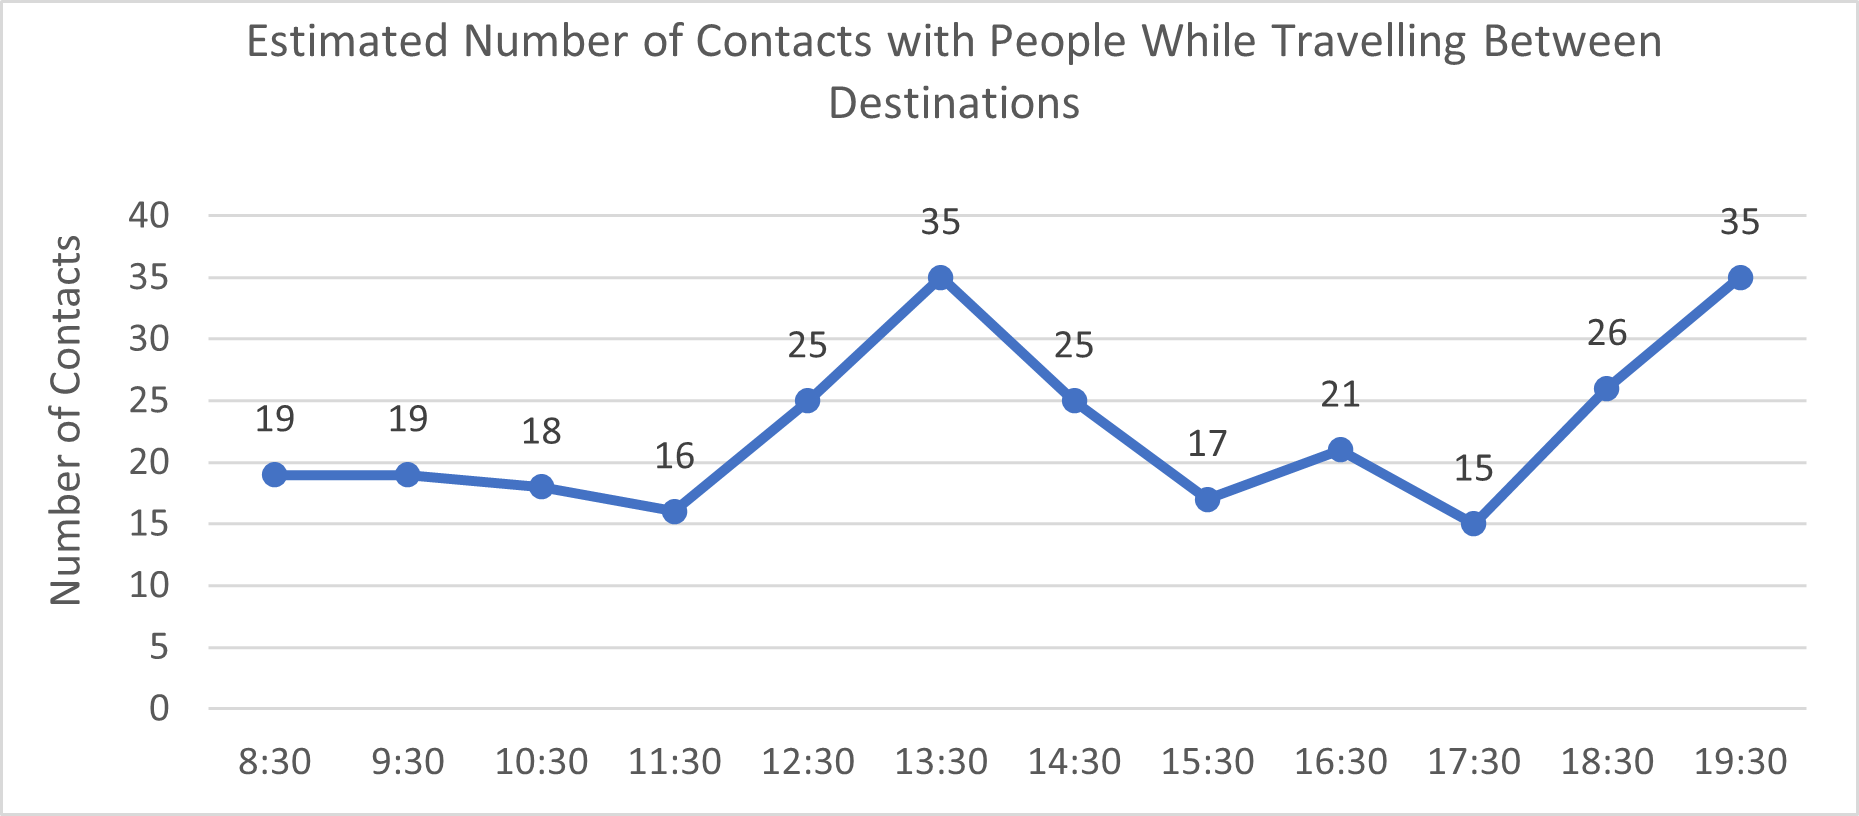
\includegraphics[width=0.8\textwidth]{figures/contact_control.png}}
    \caption{Control for number of contacts in TEST-2, created using excel.}
    \label{fig:control_contacts}
\end{figure}